\documentclass[mathNotesPreamble]{subfiles}
\begin{document}
% \relscale{1.4} %TODO
\section{14.1: Vector-Valued Functions}

  Vector-valued functions are functions of the form $\vecr(t)=\bracket{x(t),y(t),z(t)}$, where $x(t)$, $y(t)$, and $z(t)$ are parametric equations dependent on $t$.
  
  \begin{center}
    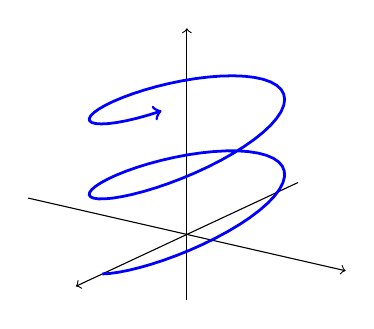
\begin{tikzpicture}
      \begin{axis}[
        axis lines=center,
        axis line style={black,->},
        xmin=-4.5, xmax=4.5,
        ymin=-2.5, ymax=2.5,
        zmin=-0.125, zmax=2,
        xmajorticks=false,
        ymajorticks=false,
        zmajorticks=false,
        enlargelimits={abs=0.75},
        view={125}{25},
        every axis plot/.append style={line width=0.5pt, color=blue}
        ]
        \addplot3[domain=0:4.25*pi, samples=100, samples y=0, ->, line width=1pt] ({4*cos(deg(x))},{sin(deg(x))},{x/6.28}); 
      \end{axis}
    \end{tikzpicture}
  \end{center}
  
  \textbf{Curves in Space}\\
  Consider 
    \[\vecr(t)=\bracket{f(t),g(t),h(t)}=f(t)\bfi+g(t)\bfj+h(t)\bfk,\]
  where $f$,\ $g$, and $h$ are defined for $a\leq t\leq b$. The
  \textbf{domain} of $\vecr$ is the largest set of $t$ for which all of
  $f$,\ $g$, and $h$ are defined.
  \vspace*{\baselineskip}

  \begin{ex*}
    What plane does the curve $\vecr(t)=t\bfi+6t^3\bfk$ lie?
  \end{ex*}
  \vspace*{\stretch{1}}

  \begin{ex*}[Lines as vector-valued functions]
    Find a vector function for the line that passes through the points $P(5,2,-4)$ and $Q(5,5,-2)$. What about the line segment that connects $P$ and $Q$?
  \end{ex*}
  \vspace*{\stretch{1}}
  \pagebreak

  \begin{ex*}
    Find the domain of
      \[\vecr(t)=\sqrt{16-t^2}\bfi+\sqrt{t}\bfj+\frac{4}{\sqrt{3+t}}\bfk\]
  \end{ex*}
  \vspace*{\stretch{1}}

  \begin{ex*}
    Find the point $P$ on 
      \[\vecr(t)=t^2\bfi+2t\bfj+2t\bfk,\]
    closest to $P_0(4,17,10)$. What is the distance between $P$ and $P_0$?
  \end{ex*}
  \vspace*{\stretch{1}}
  \pagebreak

  \textbf{Orientation of Curves}\\
  \begin{itemize}
    \item A \textbf{unparameterized curve} is a smooth curve $C$ with no specified direction and the tangent vector can be drawn in two directions.
    \item A \textbf{parameterized curve} is a smooth curve $C$ described by a function $\vecr(t)$ for $a\leq t\leq b$ and has a direction referred to as its \textbf{orientation}.
    \item The \textit{positive} orientation is the direction of the curve generated when $t$ increases from $a$ to $b$. 
    \item The tangent vector of a parameterized curve points in the positive orientation of the curve.
  \end{itemize}
  \vspace*{\stretch{1}}
  \begin{center}
    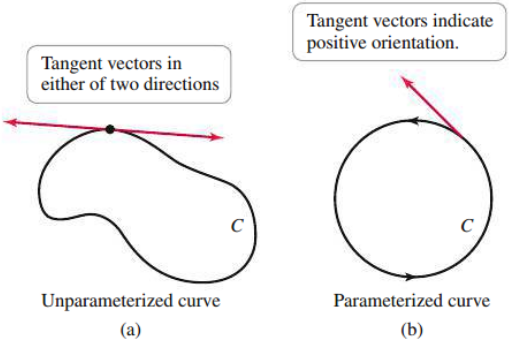
\includegraphics[width=0.65\linewidth]{images/briggs_14_01/fig14_03}
  \end{center}
  \vspace*{\stretch{1}}
  \pagebreak

  \begin{ex*}
    Graph the curve described by the equation
      \[\vecr(t)=4\cos(t)\bfi+\sin(t)\bfj+\frac{t}{2\pi}\bfk,\]
    where $0\leq t\leq 2\pi$. Indicate the positive orientation of this curve.
  \end{ex*}
  \pagebreak

  \textbf{Limits and Continuity for Vector-Valued Functions}\\
    The properties of limits extend to vector-valued functions naturally. In particular, for $\vecr(t)=\bracket{f(t), g(t), h(t)}$, if
      \[\lim_{t\to a} f(t)=L_1, \qquad \lim_{t\to a} g(t)=L_2, \qquad \lim_{t\to a} h(t)=L_3\]
    then
      \[\lim_{t\to a} \vecr(t)=\bracket{\lim_{t\to a} f(t),\ \lim_{t\to a} g(t),\ \lim_{t\to a} h(t)}=\bracket{L_1,L_2,L_3}.\]
  \begin{defn*}[Limit of a Vector-Valued Function]
    A vector-valued function $\vecr$ approaches the limit $\mathbf L$ as $t$ approaches $a$, written \newline$\displaystyle\lim_{t\to a} \vecr(t)=\mathbf L$, provided $\displaystyle\lim_{t\to a}\abs{\vecr(t)-\mathbf L}=0$.
    \vspace*{\baselineskip}
    
    A function $\vecr(t)$ is \textbf{continuous} at $t=a$, provided $\displaystyle \lim_{t\to a} \vecr(t)=\vecr(a)$.
  \end{defn*}

  \begin{ex*}
    Evaluate the following limits:
    \begin{tasks}[after-item-skip=\stretch{1}, label=](1)
      \task 
        $\displaystyle \lim_{t\to \pi} \parens{\cos(t)\bfi-7\sin\parens{-\frac{t}{2}}\bfj+\frac{t}{\pi}\bfk}$
      \task 
        $\displaystyle \lim_{t\to \infty} \parens{\frac{t}{t-3}\bfi+\frac{40}{1+19e^{-t}}\bfj+\frac{1}{2t}\bfk}$
    \end{tasks}
    \vspace*{\stretch{1}}
  \end{ex*}

  \pagebreak
  
\end{document}
